%************************************************
\chapter{Pre-processing High Throughput Animal Tracking Data}\label{ch:preprocessing}
%************************************************
% 
\noindent \textbf{Pratik R. Gupte}, Christine E. Beardsworth\textsuperscript{1}, Orr Spiegel\textsuperscript{2}, Emmanuel Lourie\textsuperscript{3}, Sivan Toledo\textsuperscript{2}, Ran Nathan\textsuperscript{3}, and Allert Bijleveld\textsuperscript{1}

\marginpar{
    \textsuperscript{1} Netherlands Inst. for Sea Research, The Netherlands.
    
    \medskip
    
    \textsuperscript{2} Tel Aviv University, Israel.
    
    \medskip

    \textsuperscript{3} The Hebrew University of Jerusalem, Israel.
}

\section*{Abstract}

\footnotesize{
    Modern, high-throughput animal tracking increasingly yields `big data' at very fine temporal scales. 
    At these scales, location error can exceed the animal's step size, leading to mis-estimation of behaviours inferred from movement. 
    `Cleaning' the data to reduce location errors is one of the main ways to deal with position uncertainty. 
    Though data cleaning is widely recommended, inclusive, uniform guidance on this crucial step, and on how to organise the cleaning of massive datasets, is relatively scarce.
    A pipeline for cleaning massive high-throughput datasets must balance ease of use and computationally efficiency, in which location errors are rejected while preserving valid animal movements. 
    Another useful feature of a pre-processing pipeline is efficiently segmenting and clustering location data for statistical methods, while also being scalable to large datasets and robust to imperfect sampling. 
    Manual methods being prohibitively time consuming, and to boost reproducibility, pre-processing pipelines must be automated.
    We provide guidance on building pipelines for pre-processing high-throughput animal tracking data to prepare it for subsequent analyses. 
    We apply our proposed pipeline to simulated movement data with location errors, and also show how large volumes of cleaned data can be transformed into biologically meaningful `residence patches', for exploratory inference on animal space use. 
    We use tracking data from the Wadden Sea ATLAS system (WATLAS) to show how pre-processing improves its quality, and to verify the usefulness of the residence patch method. 
    Finally, with tracks from Egyptian fruit bats \textit{Rousettus aegyptiacus}, we demonstrate the pre-processing pipeline and residence patch method in a fully worked out example.
    To help with fast implementation of standardised methods, we developed the R package \textit{atlastools}, which we also introduce here. 
    Our pre-processing pipeline and \textit{atlastools} can be used with any high-throughput animal movement data in which the high data-volume combined with knowledge of the tracked individuals’ movement capacity can be used to reduce location errors. 
    \textit{atlastools} is easy to use for beginners, while providing a template for further development. 
    The common use of simple yet robust pre-processing steps promotes standardised methods in the field of movement ecology and leads to better inferences from data.

    \medskip

    \noindent {\large{\color{Maroon}$\Delta$}} Published in the \textit{Journal of Animal Ecology} as Gupte et al. (2021). A guide to pre-processing high throughput tracking data.
}

\clearpage

% \begin{refsection}
%     \section{Introduction}

%     The movement of an animal is an adaptive, integrated response to multiple drivers, including internal state, life-history traits and capacities, biotic interactions, and other environmental factors \cite{nathan2008a, holyoak2008}.
%     % Movement has both beneficial and detrimental consequences for individual fitness, and 
%     The movement ecology framework links the drivers, processes, and fitness outcomes of animal movement \cite{nathan2008a}, and remotely tracking individual animals in the wild is the methodological mainstay of movement ecology \cite{wikelski2007,nathan2008a,hussey2015,kays2015}.
%     A key challenge with observed tracks is to extract information on the behavioural, cognitive, social, ecological and evolutionary processes that shape animal movement.
%     Addressing this challenge requires investigating the relationships between movement and its drivers at the fine scales at which animals sense and respond to variation in their environment. 
%     Tracking data, which are observations of a continuous process (animal movement) at discrete timesteps, reveal useful information about the movement process when the tracking interval is considerably shorter than the typical duration of a movement mode \cite{nathan2008a, noonan2019, getz2008}.
%     This can be accomplished by wildlife tracking systems that collect position data from many individuals at high temporal and spatial resolution (i.e., high-throughput tracking) relative to the scale of the movement mode of interest \cite{getz2008}.
%     High-throughput tracking technologies include GPS tags \cite{strandburg-peshkin2015, papageorgiou2019, harel2016, klarevas-irby2021}, tracking radars \cite{horvitz2014}, and computer vision methods for tracking entire groups of animals from video recordings \cite{rathore2020, perez-escudero2014}. 
%     Furthermore, high-throughput wildlife tracking is routinely provided by terrestrial reverse-GPS systems such as ATLAS \cite[Advanced Tracking and Localization of Animals in real-life Systems:][]{toledo2014, weiser2016, toledo2016,toledo2020} --- see also \cite{maccurdy2009, maccurdy2019} --- and underwater acoustic reverse-GPS tracking of aquatic animals \cite{baktoft2019, baktoft2017, jung2015, aspillaga2021, aspillaga2021a}.
%     Finally, low resolution tracking over a long duration may also capture important aspects of animal behaviour at certain time-scales \cite[e.g. migration, long-range dispersal;][]{getz2008}, thereby being `relatively' high-throughput.

%     Although high-throughput tracking provides a massive amount of data on the path of a tracked animal, these data present a challenge to ecologists.
%     When tracking animals at a high temporal resolution, the location error of each position may approach or exceed the true movement distance of the animal, compared to low-resolution tracking with the same measurement error.
%     This leads to an over-estimation of the true distance moved by an animal between two discrete time-points, leading to unreliable behavioural metrics ultimately derived from movement distance, such as speed and tortuosity \cite[see][]{ranacher2016, noonan2019, hurford2009, calenge2009}.
%     Additionally, the location error around a position introduces uncertainty when studying the relationship between animal movements and either fixed landscape features (e.g. roads), or mobile elements (e.g. other tracked individuals), as well as confounding estimates of habitat selection.
%     Users have two main options to improve data quality, \textit{(i)} making inferences after modelling the system-specific location error using a continuous time movement model \cite{fleming2014a, fleming2020, jonsen2003, jonsen2005, johnson2008, patterson2008, aspillaga2021}, or \textit{(ii)} pre-processing data to clean it of positions with large location errors \cite{bjorneraas2010}.
%     The first approach may be limited by the animal movement models that can be fitted to the data \cite{fleming2014a, noonan2019, fleming2020}, may result in unreasonable computation times, or may be entirely beyond the computational capacity of common hardware, leading users to prefer data cleaning instead.
%     Data cleaning reveals another challenge of high-throughput tracking: the large number of observations make it difficult for researchers to visually examine each animal's track for errors \cite{weiser2016, toledo2020}.
%     With manual identification and removal of errors from individual tracks prohibitively time consuming, data cleaning can benefit from automation based on a protocol.

%     Pre-processing of movement data --- defined as the set of data management steps executed prior to data analysis --- must reliably discard large location errors, also called outliers, from tracks (analogous to reducing false positives) while avoiding the overzealous rejection of valid animal movements (analogous to reducing false negatives).
%     How well researchers balance these imperatives has consequences for downstream analyses \cite{stine2001}.
%     For instance, small-scale resource selection functions can easily infer spurious preference and avoidance effects when there is uncertainty about an animal's true position \cite{visscher2006}.
%     Ecologists recognise that tracking data are imperfect observations of the underlying movement process, yet they implicitly consider cleaned data equivalent to the ground-truth.
%     This assumption is reflected in popular statistical methods in movement ecology such as Hidden Markov Models (HMMs) \cite{langrock2012}, stationary-phase identification methods \cite{patin2020a}, or step-selection functions (SSFs) \cite{barnett2008, signer2017, avgar2016}, which expect minimal location errors relative to real animal movement (i.e., a high signal-to-noise ratio).
%     This makes the reproducible, standardised removal of location errors crucial to any animal tracking study.
%     While gross errors are often removed by positioning-system algorithms in both GPS and reverse-GPS setups, `reasonable’ errors often remain to confront end users \cite{fischler1981, weiser2016, ranacher2016}.
%     Further, as high-throughput tracking is deployed in more regions and for more species, standardised pre-processing steps should be general enough to tackle animal movement data recovered from a range of environments, so as to enable sound comparisons across species and ecosystems.

%     Despite the importance and ubiquity of reducing location errors in tracking data, movement ecologists lack formal guidance on this crucial step.
%     Pre-processing protocols are not often reported in the literature, or may not be easily tractable for mainstream computing hardware and software.
%     Some tracking data, such as GPS, are autonomously pre-processed without user access to the raw data \cite[using error estimates and Kalman smooths;][and substantial location errors may yet persist]{kaplan2005}.
%     However, filtering out positions using estimates of location error alone may not be sufficient to exclude outliers which represent unrealistic movement but have low error measures \cite{weiser2016, ranacher2016}.
%     When tracking systems do make their raw data available to researchers, this can enable users to better control the data pre-processing stage, and to substantially improve data quality while ensuring that cleaning does not itself lead to unrealistic movement tracks \cite[e.g. Kalman smooths which distort tracks,][]{kaplan2005}.
%     Furthermore, 
%     This makes identifying and removing biologically implausible locations from a track an important component of recovering true animal movement \cite{bjorneraas2010}.
%     Even after removing unrealistic movement, a track may be comprised of positions that are randomly distributed around the true animal location \cite{noonan2019}.
%     The large data-volumes of high-throughput tracking allow for a neat solution: tracks can be `median smoothed' to reduce small location errors that have remained undetected \cite[e.g.][]{bijleveld2016} 
%     Large data volumes may also need to be thinned, for example, examining environmental covariates as predictors of prolonged residence in an area  \cite[see e.g.][]{bracis2018, aarts2008, bijleveld2016, oudman2018, harel2016} might require thinning of high-resolution movement data to match the lower spatial resolution of environmental measurements. 
%     Data thinning and clustering are also required to avoid non-independent observations due to strong spatio-temporal autocorrelation, or to examine the effect of sampling scale on movement metrics and resource-selection \cite{fleming2014a,noonan2019}.

%     When dealing with datasets that contain many millions of positions, reseachers may run into computational limits when trying to apply pre-processing steps to their full dataset.
%     For instance, the size of working memory (RAM) limits the size of datasets that can be loaded into \textit{R}, the programming and statistical language of choice in movement ecology \cite{r2020,joo2020,joo2020b}.
%     Data-rich fields such as genomics inspire a possible solution: to break very large data into smaller subsets, and pass these subsets through automated computational `pipelines' \cite{schadt2010,peng2011}.
%     Pre-processing pipelines for animal tracking data --- the set of steps that users apply to prepare the data for a specific analysis --- come with some additional concerns: \textit{(i)} identifying which pre-processing steps are necessary, and \textit{(ii)} ensuring that these steps reproducibly operate on the data as expected, and as efficiently as possible.
%     While exploratory data analysis and visualisation can help determine how to pre-process the data to maximise the signal to noise ratio \cite{slingsby2016}, standardising implementations of pre-processing techniques into robust, version controlled software packages \cite[e.g. in \textit{R}, see]{wickham2015}, can increase the reliability and reproducibility of animal movement ecology \cite{haddaway2015,archmiller2020,powers2019,lewis2018}.
%     Overcoming hard computational constraints on speed and memory usage for very large data will often require a combination of programming strategies, such as using tools optimised for tabular data, or parallelised processing.

%     Here, we present guidelines for reproducibly pre-processing high-throughput animal tracking data (Fig. 1), with a focus on simple, widely generalisable steps that help improve data quality (Fig. 2).
%     We take two important considerations into account, that \textit{(i)} the pre-processing steps should be easily understood and reproduced, and \textit{(ii)} our implementations must be computationally efficient and reliable.
%     Consequently, formalising tools as functions in an \textit{R} package would improve portability and reproducibility \cite{marwick2018, wickham2015}.
%     Using simulated movement tracks, we demonstrate simple yet robust implementations of the pre-processing steps we recommend, conveniently wrapped into the \textit{R} package \textit{atlastools} \cite{gupte2020a}, with a discussion of features that make these steps more reproducible, and more efficient.
%     We also suggest one potential application of high-throughput tracking in studies of animal movement and space use, illustrated by the first-principles based synthesis of `residence patches' from clusters of spatio-temporally proximate positions \cite[\textit{sensu}][]{bijleveld2016, oudman2018, barraquand2008}.
%     In two fully worked out examples using our package on real tracking data, we show how to apply basic spatio-temporal and data quality filters, how to filter out unrealistic movement, and how to reduce the effect of location error with a median smooth.
%     In the first example, using calibration data from an ATLAS system, we show how the residence patch segmentation-clustering method can be used to accurately identify areas of prolonged residence under real field conditions.
%     Finally, in our second example, we use ATLAS data from Egyptian fruit bats (\textit{Rousettus aegyptiacus}) tracked in the Hula Valley, Israel, to show a fully worked out example of the pre-processing pipeline and the residence patch method.
%     While our approach to high-throughput tracking data, and our package of pre-processing functions was developed with reverse-GPS ATLAS systems in mind, both are broadly suitable to a wide range of high-throughput animal tracking data sources, from underwater acoustic reverse-GPS \cite{baktoft2019, baktoft2017, jung2015, aspillaga2021, aspillaga2021a}, high-resolution GPS \cite{strandburg-peshkin2015, papageorgiou2019, harel2016, klarevas-irby2021}, tracking radars \cite{horvitz2014}, and visual video tracking \cite{rathore2020, perez-escudero2014}.

%     \section{Best-Practices for Pre-Processing Workflows}

%     % \begin{figure}
%     %     \centering
%     %     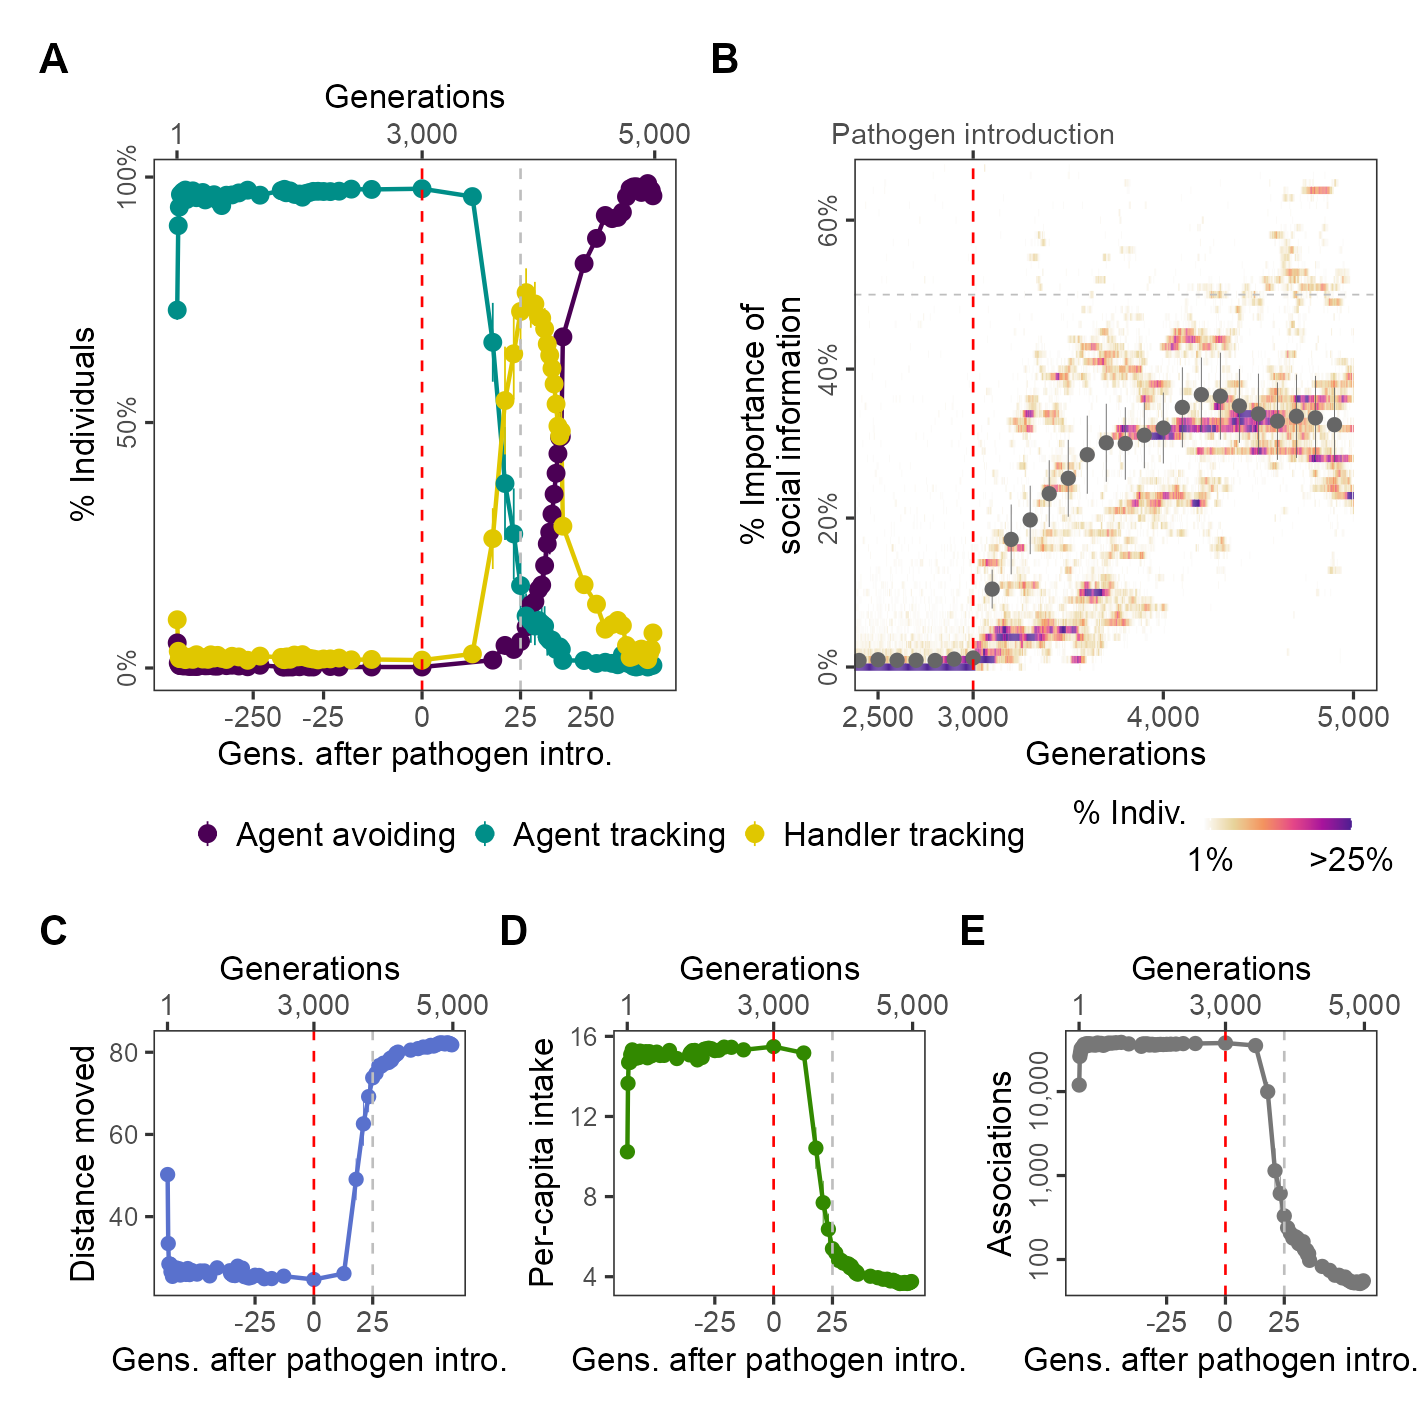
\includegraphics[width=0.95\textwidth]{figures/fig_01.png}
%     %     \caption{
%     %         \textbf{Some best-practices for pre-processing high-throughput tracking data.}\\
%     %         Simple pre-processing of animal tracking data can improve the quality of animal tracking data, and the inferences that are drawn from it.
%     %         The organisation of pre-processing workflows into a `pipeline' --- a set of steps that users apply to prepare the data for a specific analysis --- can help make research more reproducible and reliable.
%     %         Exploratory data analysis of representative subsets of the data can help to identify common issues with data quality, and to determine which pre-processing, steps such as filters and smooths, might be necessary (\textit{see also Fig. 2}).
%     %         Pre-processing steps implemented as programming code can be made reproducible and shareable by following best-practices for software development: (1) tracking changes to the steps, and the software used, using version control (e.g. \textit{git}, \textit{renv}), (2) preferring pre-existing tools, such as \textit{R} packages, which are well documented and tested, (3) encapsulating custom-written code as functions, and bundling related functions into a package, and (4) checking the quality of both custom-written code (e.g. by testing functions), and the overall pipeline (e.g. data visualisation).
%     %         The efficiency of pre-processing steps can be increased by using strategies for dealing with large datasets, such as batch processing, or using a computing cluster.
%     %         The use of existing tools optimised for large datasets, or by writing code in a `fast' language such as \textit{C++}, can also speed up the pre-processing of large datasets (see main text for examples).
%     %         See the \textsc{Worked Out Example} on Egyptian fruit bats, as well as Supplementary Material 1, for more details on implementing pipelines.
%     %         Fig. 2 shows an example of such a pipeline.
%     %     }
%     %     \label{fig:figure_concept}
%     % \end{figure}

%     \subsection{Exploratory Data Analysis to Identify Pre-processing Steps}

%     Exploratory data analysis should be the first step towards pre-processing movement data \cite[see Fig. 1;][]{slingsby2016}.
%     Researchers with very large datasets of perhaps millions of rows should ideally select a representative subset of these data for exploratory data analysis, including individuals of different species, sexes, or seasonal cohorts.
%     Examples of exploratory data analysis include plotting heatmaps of the number of observations per unit area across the study site (Fig. 1).
%     Histograms of the location error estimates, plotting the linear approximations of animal paths between observations, and histograms of the sampling interval can help determine how data need to be treated so as to minimise location errors and improve computational tractability (Fig. 1).
%     While pre-processing steps required for datasets will differ between studies and tracking technologies, we elaborate upon candidate steps and their parameterisation in following sections (see also Fig. 2).

%     \subsection{Improving Reliability and Reproducibility}

%     Following exploratory data analysis and the parameterisation of data cleaning steps, the specific implementation of these steps should be made reliable and reproducible.
%     Since reproducing pre-processing steps can be challenging when using only written descriptions from published articles, providing the code to implement pre-processing steps reduces ambiguity and increases reproducibility \cite{haddaway2015}.
%     For technically advanced users, the best-practices here are \textit{(1)} to implement pre-processing steps as `functions', \textit{(2)} to collect related functions --- e.g. for similar kinds of data --- into a software `package', \textit{(3)} to `test' that the functions handle input as expected, and \textit{(4)} implement `version control' throughout, such that the process of development is documented \cite[Fig. 1;][]{wickham2015,alston2020,perez-riverol2016}.
%     As an example, our \textit{atlastools} package incorporates these best-practices, and may be used as a reference \cite[][]{gupte2020a}.
%     We have written each pre-processing step as a separate function, and each of these functions is tested, usually on simulated data, but in some cases also on empirical data \cite[][see the directory \textit{tests/} in the associated Zenodo repository]{wickham2015}.
%     % The tests include `use cases', i.e., ensuring the functions perform calculations correctly, but also `abuse cases', which check that the functions handle unexpected inputs usefully, such as by printing informative error messages.
%     Finally, logging error messages is crucial when passing data through a pipeline, helping determine which data subsets could not be handled as expected, and why.
%     Users who would prefer to rely on pre-existing toolsets and methods can use \textit{R} packages that follow these best-practices, such as \textit{move} \cite{kranstauber2011}, and \textit{sftrack} \cite{boone2020}.

%     \subsection{Improving Speed and Efficiency}

%     The large size of modern, high-throughput animal tracking data means that the computational challenge can often be \textit{the} main challenge in working with these data.
%     For beginning users, organising their workflows so that they process subsets of the data (such as one individual) at a time can help overcome limitations on working memory.
%     Animal tracking data stored in a relational database \cite[e.g. SQL databases][]{codd1970}, for example, can be broken into meaningful subsets based on individual identity and tracking season.
%     These smaller subsets can then be loaded into working memory, pre-processed, and saved in a separate location (see Supplementary Material 1, Section 2 for a worked out example on an SQL database).
%     Using existing tools optimised for tabular data, such as the \textit{R} package \textit{data.table} \cite{dowle2020}, can also speed up computation; \textit{atlastools} is built using \textit{data.table} for this reason.
%     More advanced users seeking substantial speed gains might wish to look into parallel-processing, and process each subset of the data independently of the full dataset, for example by using a computing cluster \cite[see also][for an alternative]{zjdai2021}.
%     Finally, another advanced method, used by popular packages such as \textit{move} \cite{kranstauber2011} and \textit{recurse} \cite{bracis2018}, is to write one's own methods in a `fast' low-level language, such as \textit{C++}, and link these to \textit{R} \cite[][]{eddelbuettel2013}; see also \textit{adehabitatLT}, which is written partially in \textit{C}: \cite{calenge2006}.
%     Beginning practitioners can organise their workflows around these packages to benefit from the features they incorporate.

%     \printbibliography[heading=subbibliography]
% \end{refsection}
